\section{Background}
\label{sec:background}
This paragraph will give background information on software metrics used in this study and on the software maintainability model of SIG.

\subsection{Software Metrics}
Software metrics are quantitative measures representing certain properties of a software system. Some very basic metrics, which get aggregated in different ways to higher-level as described in the following paragraph are listed in Table \ref{tab:base_metrics}.:
\begin{table}[htbf]
\caption{Base metrics} 
\label{tab:base_metrics}
\centering
\begin{tabular}{p{0.30\linewidth} p{0.60\linewidth}}\\
Metric   &  Description\\ 
Lines of code 		&  The number of lines of code that make up the system. \\ 
Lines of comments 	&  The number of lines of comments in the code. \\
Component count		&  The number of components making up the system. \\
Cloned lines 		&  The amount of code that is present multiple times in the code. SIG defines this as a duplicate block of code longer than 6 lines. \\ 
New lines 			&   The number of lines that were not in the code in the previous snapshot.   \\
Deleted lines 		&   The number of lines that are no longer in the system but were in the previous snapshot.  \\ 
Changed lines 		&   The number of lines that are different from the previous snapshot.   \\  
Decision density 	&   Also called cyclomatic density. This refers to the McCabe complexity normalized over the length of the program. The McCabe complexity counts the number of independent linear paths through a program. \\ 
Typecount 			&   The number of programming languages that make up the system. \\
Typeset 			&   A vector containing the programming languages that make up the system. \\
No. of man months 	&   Effort it would require to rebuild the system, depending on system size and programming languages used. \\
\end{tabular}
\end{table}

\subsection{Software Maintainability Model}
SIG uses basic metrics like lines of code or McCabe's complexity and aggregates them to metrics with a higher expressiveness based on SIG's expertise \cite{heitlager2007practical} and the ISO/IEC 25010 standard \cite{iso25010}. Figure \ref{fig:mmodel} gives an overview about the aggregated metrics used in the software maintainability model. 
Volume is derived from lines of code and a productivity factor for the corresponding language (see \cite{jones1996programming}). Duplication is based on duplicated and redundant lines of code and code complexity based on the distribution of decision density among all underlying units of a system. More insight is given by Heitlager et. al, 2007. 
Those metrics are again aggregated according to ISO/IEC 25010 as shown in Figure \ref{fig:mmodel} and form the sub-characteristics of software maintainability. All of those metrics are star-ratings ranging from 0.5 to 5.5 stars on a continuous scale, where a higher rating stands for better quality. The resulting maintainability rating is also a star rating ranging from 0.5 to 5.5 and is modeled in a way that the distribution of ratings over all systems is approaching a normal distribution. The maintainability rating can be considered as most representative for the code quality of a software system and is therefore used as equivalent for the system's quality.

\begin{figure}[!htb]
  \centering
  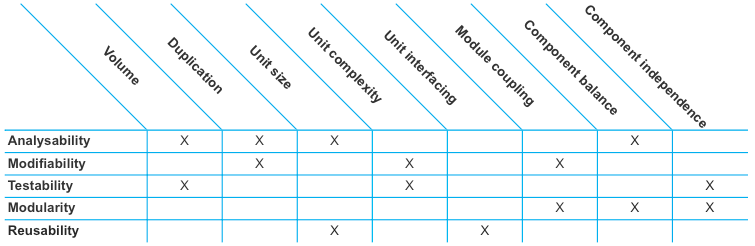
\includegraphics[width=1\linewidth]{figs/mmodel.png}
  \caption{Maintainability model}
  \label{fig:mmodel}
\end{figure}

%%% Local Variables:
%%% mode: latex
%%% TeX-master: "IWSM-Mensura-2016"
%%% End:
